\chapter{Manual de Usuario para el Administrador}
\label{chap:manadmin}

El administrador será el responsable de la gestión de la plataforma y el encargado de dar de baja y añadir nuevos administradores y docentes en la base de datos. Por tanto, deberá conocer de una manera adecuada los procedimientos a realizar en cada uno de los casos o tareas que deba desempeñar. Este usuario tendrá acceso al proyecto de Firebase, cuya página inicial se muestra en la Figura \ref{fig:maniniciofirebase}.

\begin{figure}[!h]
	\begin{center}
		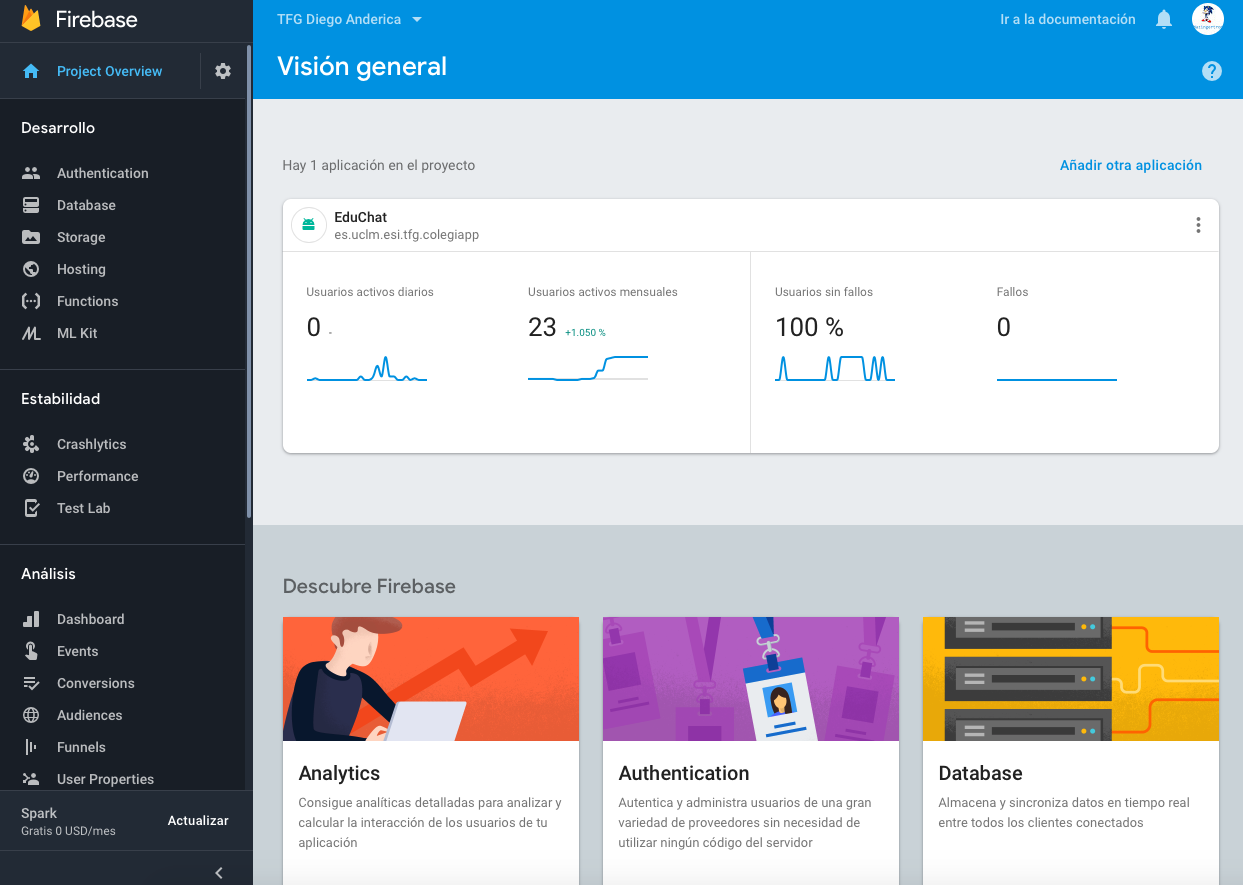
\includegraphics[width=0.95\textwidth]{/manuales/administrador/inicio_firebase}
		\caption{Página de Inicio del Proyecto de Firebase}
		\label{fig:maniniciofirebase}
	\end{center}
\end{figure}

\clearpage

En la columna lateral izquierda se encuentran todas las funciones que puede ofrecer la plataforma de Google, aunque primero se hablará de \textit{Database}, que se trata de la base de datos no relacional donde se alojará la mayor parte de la información. Una vez que el administrador se haya dirigido a este apartado, se mostrará una página Web con la información de la base de datos organizada en colecciones (Figura \ref{fig:iniciobbdd}). A continuación, se explicará cómo añadir nuevos docentes, así como nuevos administradores.

\begin{figure}[!h]
	\begin{center}
		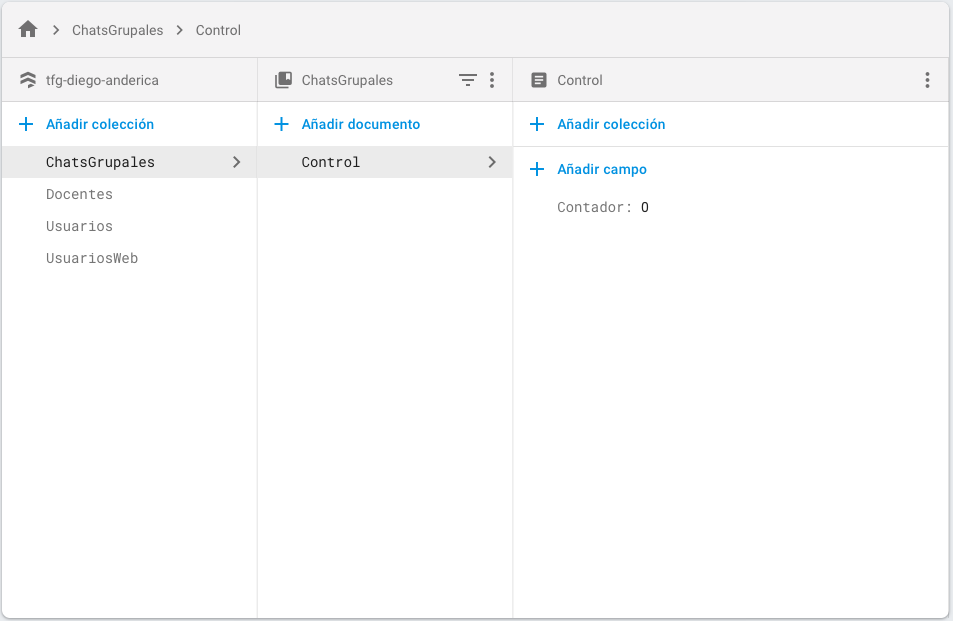
\includegraphics[width=0.95\textwidth]{/manuales/administrador/inicio_bbdd}
		\caption{Página de Inicio de la Base de Datos}
		\label{fig:iniciobbdd}
	\end{center}
\end{figure}

\clearpage

\section*{Añadir un Nuevo Docente}
En el caso de que un administrador desee dar de alta a un nuevo docente, bastará con dirigirse a la colección <<Docentes>>, haciendo clic sobre ella. El sitio Web mostrará todos los documentos existentes que representan a cada uno de los docentes registrados (Figura \ref{fig:bbdddocentes}). Posteriormente, deberá pulsar sobre el botón <<Añadir documento>>, que se encuentra situado en la columna central para comenzar el procedimiento. Se abrirá un nuevo formulario (Figura \ref{fig:adddocente}), donde el administrador podrá comenzar a rellenar los campos que se muestran en el ejemplo de la Figura \ref{fig:bbdddocentes} con la información del nuevo docente, haciendo clic sobre el botón <<Añadir campo>> para introducir nuevos campos. El tipo en todos los campos deberá ser \textit{String}.

\begin{figure}[!h]
	\begin{center}
		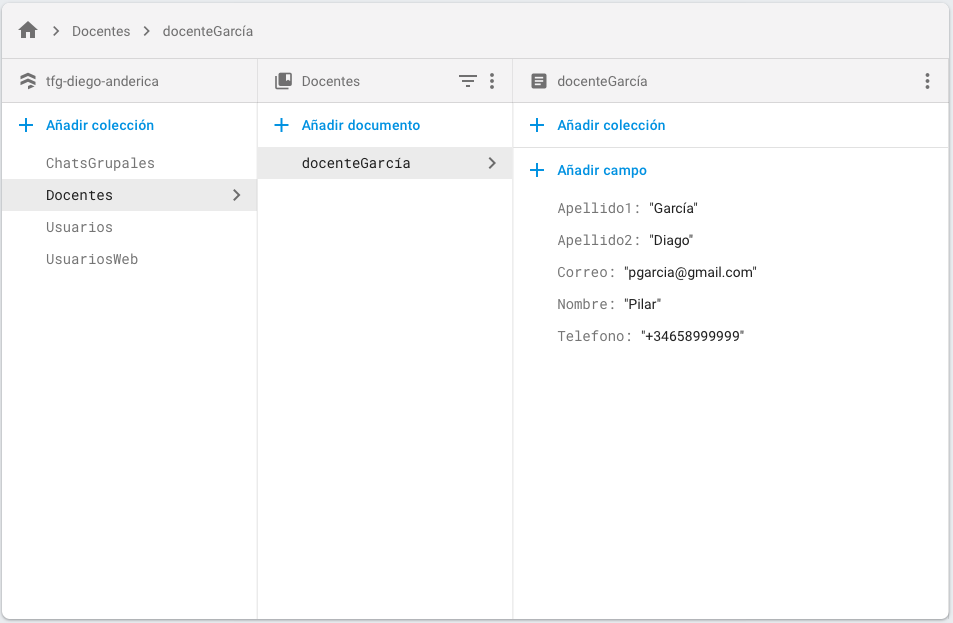
\includegraphics[width=0.7\textwidth]{/manuales/administrador/bbdd_docentes}
		\caption{Ejemplo Colección Docentes}
		\label{fig:bbdddocentes}
	\end{center}
\end{figure}

\begin{figure}[!h]
	\begin{center}
		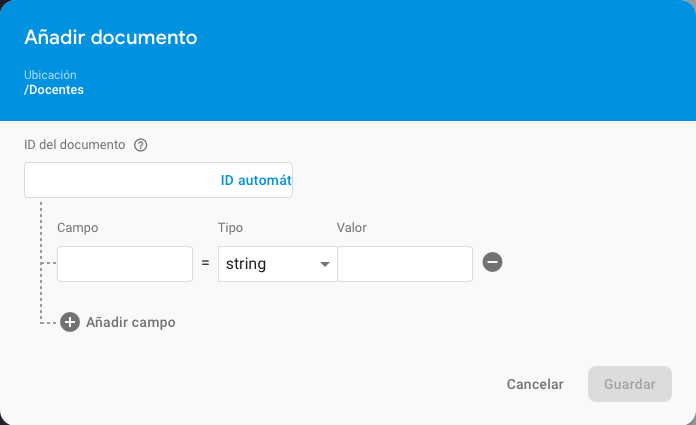
\includegraphics[width=0.7\textwidth]{/manuales/administrador/add_docente}
		\caption{Añadir Nuevo Documento}
		\label{fig:adddocente}
	\end{center}
\end{figure}

\clearpage

Un ejemplo en el que se añadiría un nuevo docente es el que se muestra en la Figura \ref{fig:errordocente}, donde el campo <<ID del documento>> deberá rellenarse (sin tildes para una mayor consistencia) con la estructura \mbox{\textit{docentePrimerApellidoX}}, siendo X un número, en caso de que ya exista otro docente con el mismo identificador, situación que será advertida (Figura \ref{fig:errordocente}).

\begin{figure}[!h]
	\begin{center}
		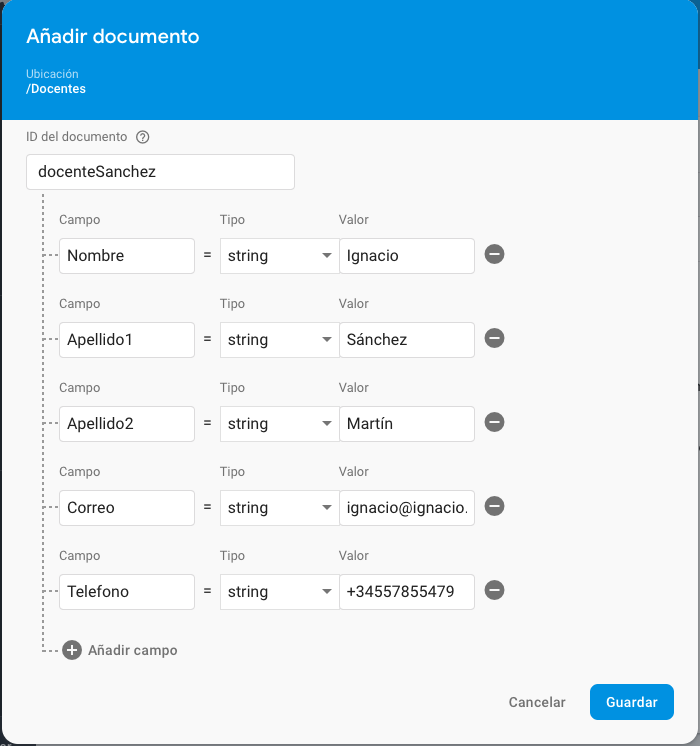
\includegraphics[width=0.7\textwidth]{/manuales/administrador/ejemplodocente}
		\caption{Ejemplo de Creación de un Nuevo Docente}
		\label{fig:ejemploocente}
	\end{center}
\end{figure}

\begin{figure}[!h]
	\begin{center}
		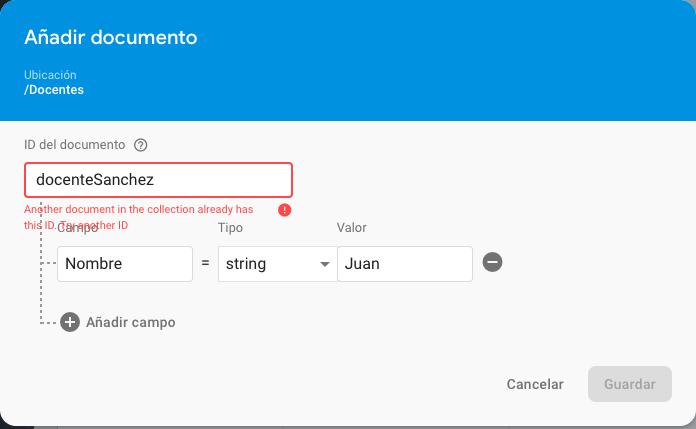
\includegraphics[width=0.7\textwidth]{/manuales/administrador/errordocente}
		\caption{Documento Existente}
		\label{fig:errordocente}
	\end{center}
\end{figure}

Una vez finalizado el proceso, se debe hacer clic en el botón <<Guardar>>, situado en el borde inferior derecho, quedando registrado el nuevo docente en la base de datos (Figura \ref{fig:finadddocente}).

\begin{figure}[!h]
	\begin{center}
		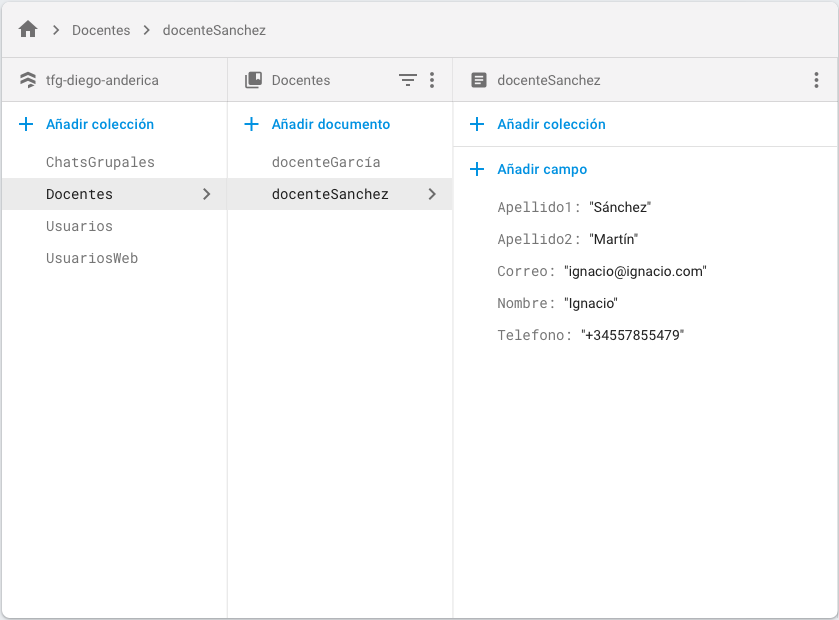
\includegraphics[width=0.75\textwidth]{/manuales/administrador/finadd_docente}
		\caption{Alta de Nuevo Docente Finalizada}
		\label{fig:finadddocente}
	\end{center}
\end{figure}

\section*{Eliminar un Docente}
Al igual que se pueden registrar nuevos docentes, también es posible eliminarlos de la base de datos. Para ello, una vez en vista de la colección <<Docentes>>, si se tuviera demasiados docentes para realizar una búsqueda manual, Firebase proporciona un filtro, representado mediante un botón con tres líneas horizontales (Figura \ref{fig:filtrodocente}) para buscar documentos por cada uno de los campos, es decir, <<Nombre>>, <<Apellido1>>, <<Telefono>>, etc.

\begin{figure}[!h]
	\begin{center}
		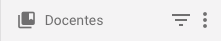
\includegraphics[width=0.4\textwidth]{/manuales/administrador/filtrodocente}
		\caption{Botón para Establecer un Filtro}
		\label{fig:filtrodocente}
	\end{center}
\end{figure}

\clearpage

Una vez que se haya encontrado el documento correspondiente al docente que se desea eliminar, bastará con seleccionarlo y abrir el menú que se encuentra en la tercera columna, haciendo clic sobre el botón con tres puntos alineados verticalmente y seleccionar la opción <<Eliminar documento>> (Figura \ref{fig:eliminardocente}). La página Web avisará de que se desea borrar ese documento y, una vez confirmada la acción, el docente será eliminado definitivamente de la base de datos.

\begin{figure}[!h]
	\begin{center}
		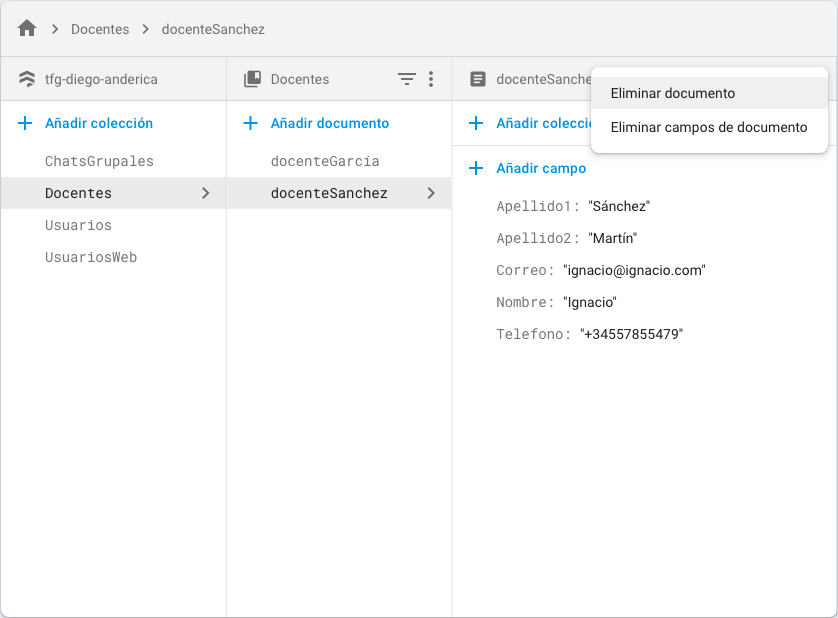
\includegraphics[width=0.7\textwidth]{/manuales/administrador/eliminardocente}
		\caption{Eliminar Docente}
		\label{fig:eliminardocente}
	\end{center}
\end{figure}

\clearpage

\section*{Añadir un Nuevo Administrador}
Los administradores también tendrán la capacidad de añadir nuevos administradores mediante la página Web de Firebase. Para ello, se deberá dirigir a la colección <<UsuariosWeb>> de la base de datos, donde se encontrarán todos los administradores actuales (Figura \ref{fig:bbdduweb}). En este caso, cada uno de los documentos tendrán únicamente dos campos: <<Correo>> y <<Contrasena>>, que son los datos requeridos para iniciar sesión en la página Web de administración.

\begin{figure}[!h]
	\begin{center}
		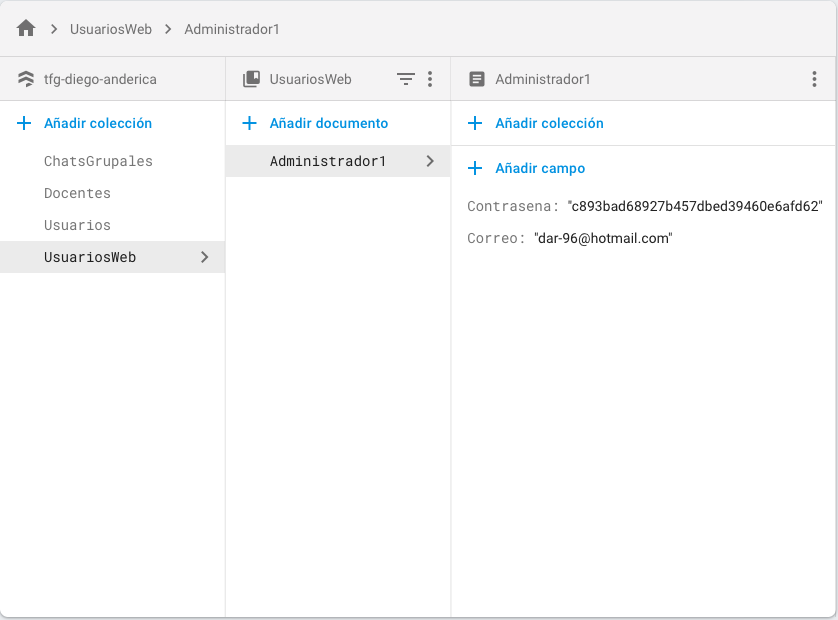
\includegraphics[width=0.7\textwidth]{/manuales/administrador/bbdd_admins}
		\caption{Colección <<UsuariosWeb>>}
		\label{fig:bbdduweb}
	\end{center}
\end{figure}

Los pasos a realizar para dar de alta a un administrador son muy similares a los que se deben seguir para dar de alta a un docente: se pulsa el botón <<Añadir documento>>, se rellenan los datos correspondientes y se pulsa el botón <<Guardar>>. En este caso, el <<ID del documento>> tendrá el formato \mbox{\textit{AdministradorX}}, siendo X un número que no se repita en la base de datos. Los datos serán proporcionados por el administrador entrante, puesto que es el único conocedor del campo <<Contrasena>>.

\section*{Eliminar un Administrador}
De igual manera a lo que se muestra en la Figura \ref{fig:eliminardocente}, se deberá seleccionar el documento del administrador a eliminar, pulsar sobre el botón de la tercera columna con tres puntos alineados verticalmente y seleccionar la opción <<Eliminar documento>>. De esta manera, se habrá eliminado un administrador de la base de datos.

\clearpage

\section*{Uso de la Página Web de Gestión}
Los administradores serán también los encargados de gestionar las familias en la base de datos, aunque esta tarea se puede realizar de una manera más cómoda desde la página Web que se ha diseñado con ese fin. Lo primero que se muestra al intentar acceder es una página de inicio de sesión (Figura \ref{fig:loginweb}), donde se deberá introducir el correo electrónico y la contraseña del administrador que, previamente, ha de estar registrado en la base de datos.

\begin{figure}[!h]
	\begin{center}
		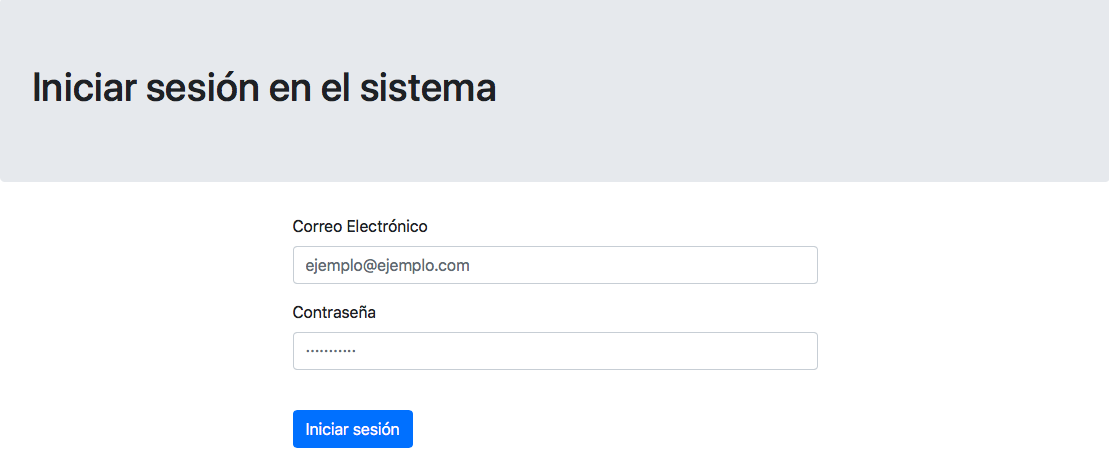
\includegraphics[width=0.8\textwidth]{/manuales/administrador/loginweb}
		\caption{Página de Inicio de Sesión}
		\label{fig:loginweb}
	\end{center}
\end{figure}

Una vez que el administrador se ha identificado correctamente, se puede comenzar a gestionar usuarios mediante una de las opciones que se muestran en la página principal: dar de alta, dar de baja, consultar o modificar usuarios (Figura \ref{fig:indexweb}). Todas estas opciones estarán disponibles de igual manera a través de la barra superior, desde donde se podrá, además, navegar hacia la página inicial haciendo clic sobre <<Gestión de Usuarios>> o cerrar la sesión mediante el botón con el mismo nombre situado en la esquina superior derecha. De aquí en adelante se explicarán cada una de las funciones principales que ofrece la página Web.

\begin{figure}[!h]
	\begin{center}
		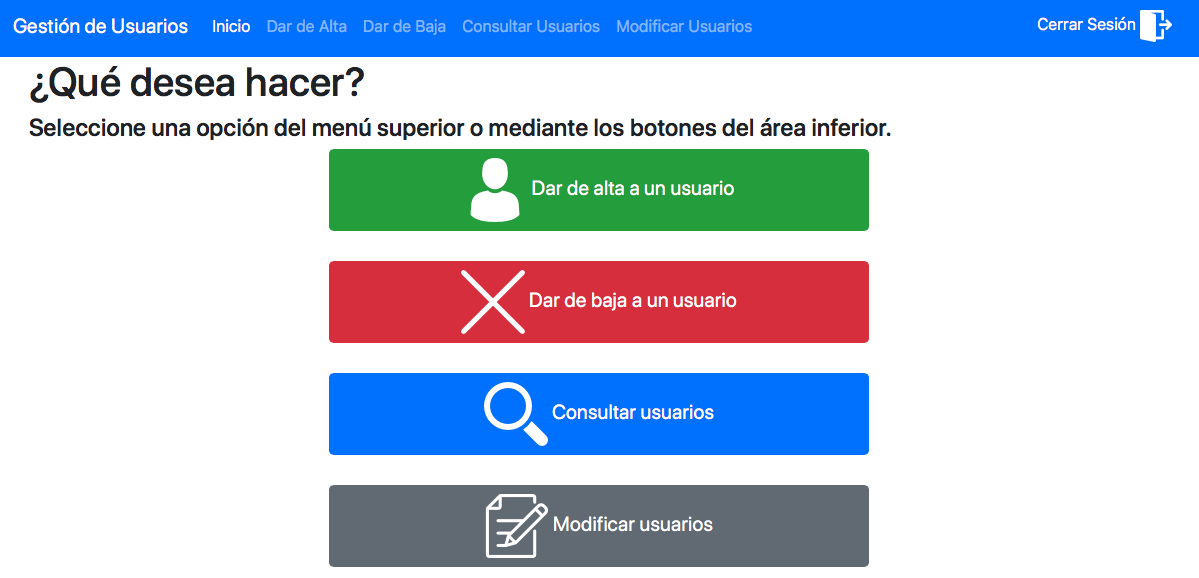
\includegraphics[width=0.8\textwidth]{/manuales/administrador/mainweb}
		\caption{Página Principal}
		\label{fig:indexweb}
	\end{center}
\end{figure}

\clearpage

\subsection*{Dar de Alta}
Al entrar en la página para dar de alta a nuevos usuarios, se tiene la posibilidad de hacerlo mediante la subida de un archivo o rellenando manualmente cada uno de los campos. Si se desea dar de alta usando un archivo con extensión \acs{CSV}, se deberá seleccionar mediante el botón <<Seleccionar archivo>> y, una vez hecho esto, pulsar sobre <<Subir Archivo>>. El navegador comenzará a realizar el registro de los usuarios en la base de datos y se notificará cuando la operación se haya completado.

Por otra parte, si se desea rellenar el formulario, se deberán especificar los campos que se encuentran disponibles. Si la familia posee dos tutores legales, se deberán habilitar los campos del segundo tutor legal pulsando sobre el botón <<Habilitar Campos Tutor 2>> (Figura \ref{fig:altaweb}). Por el contrario, si la familia únicamente posee un tutor legal, se deberán deshabilitar dichos campos pulsando sobre el mismo botón. Una vez que se tengan todos los datos introducidos, se puede pulsar sobre el botón <<Generar Nombre de Familia>> para observar en el campo <<Nombre de la familia>> con qué identificador se registrará de manera única en la base de datos, puesto que podría ser útil a la hora de realizar una consulta, aunque no es necesaria su generación por parte del administrador. En caso de que se pulse sobre el botón <<Dar de Alta Usuario/Familia>> sin haber generado su identificador, se generará automáticamente.

\begin{figure}[!h]
	\begin{center}
		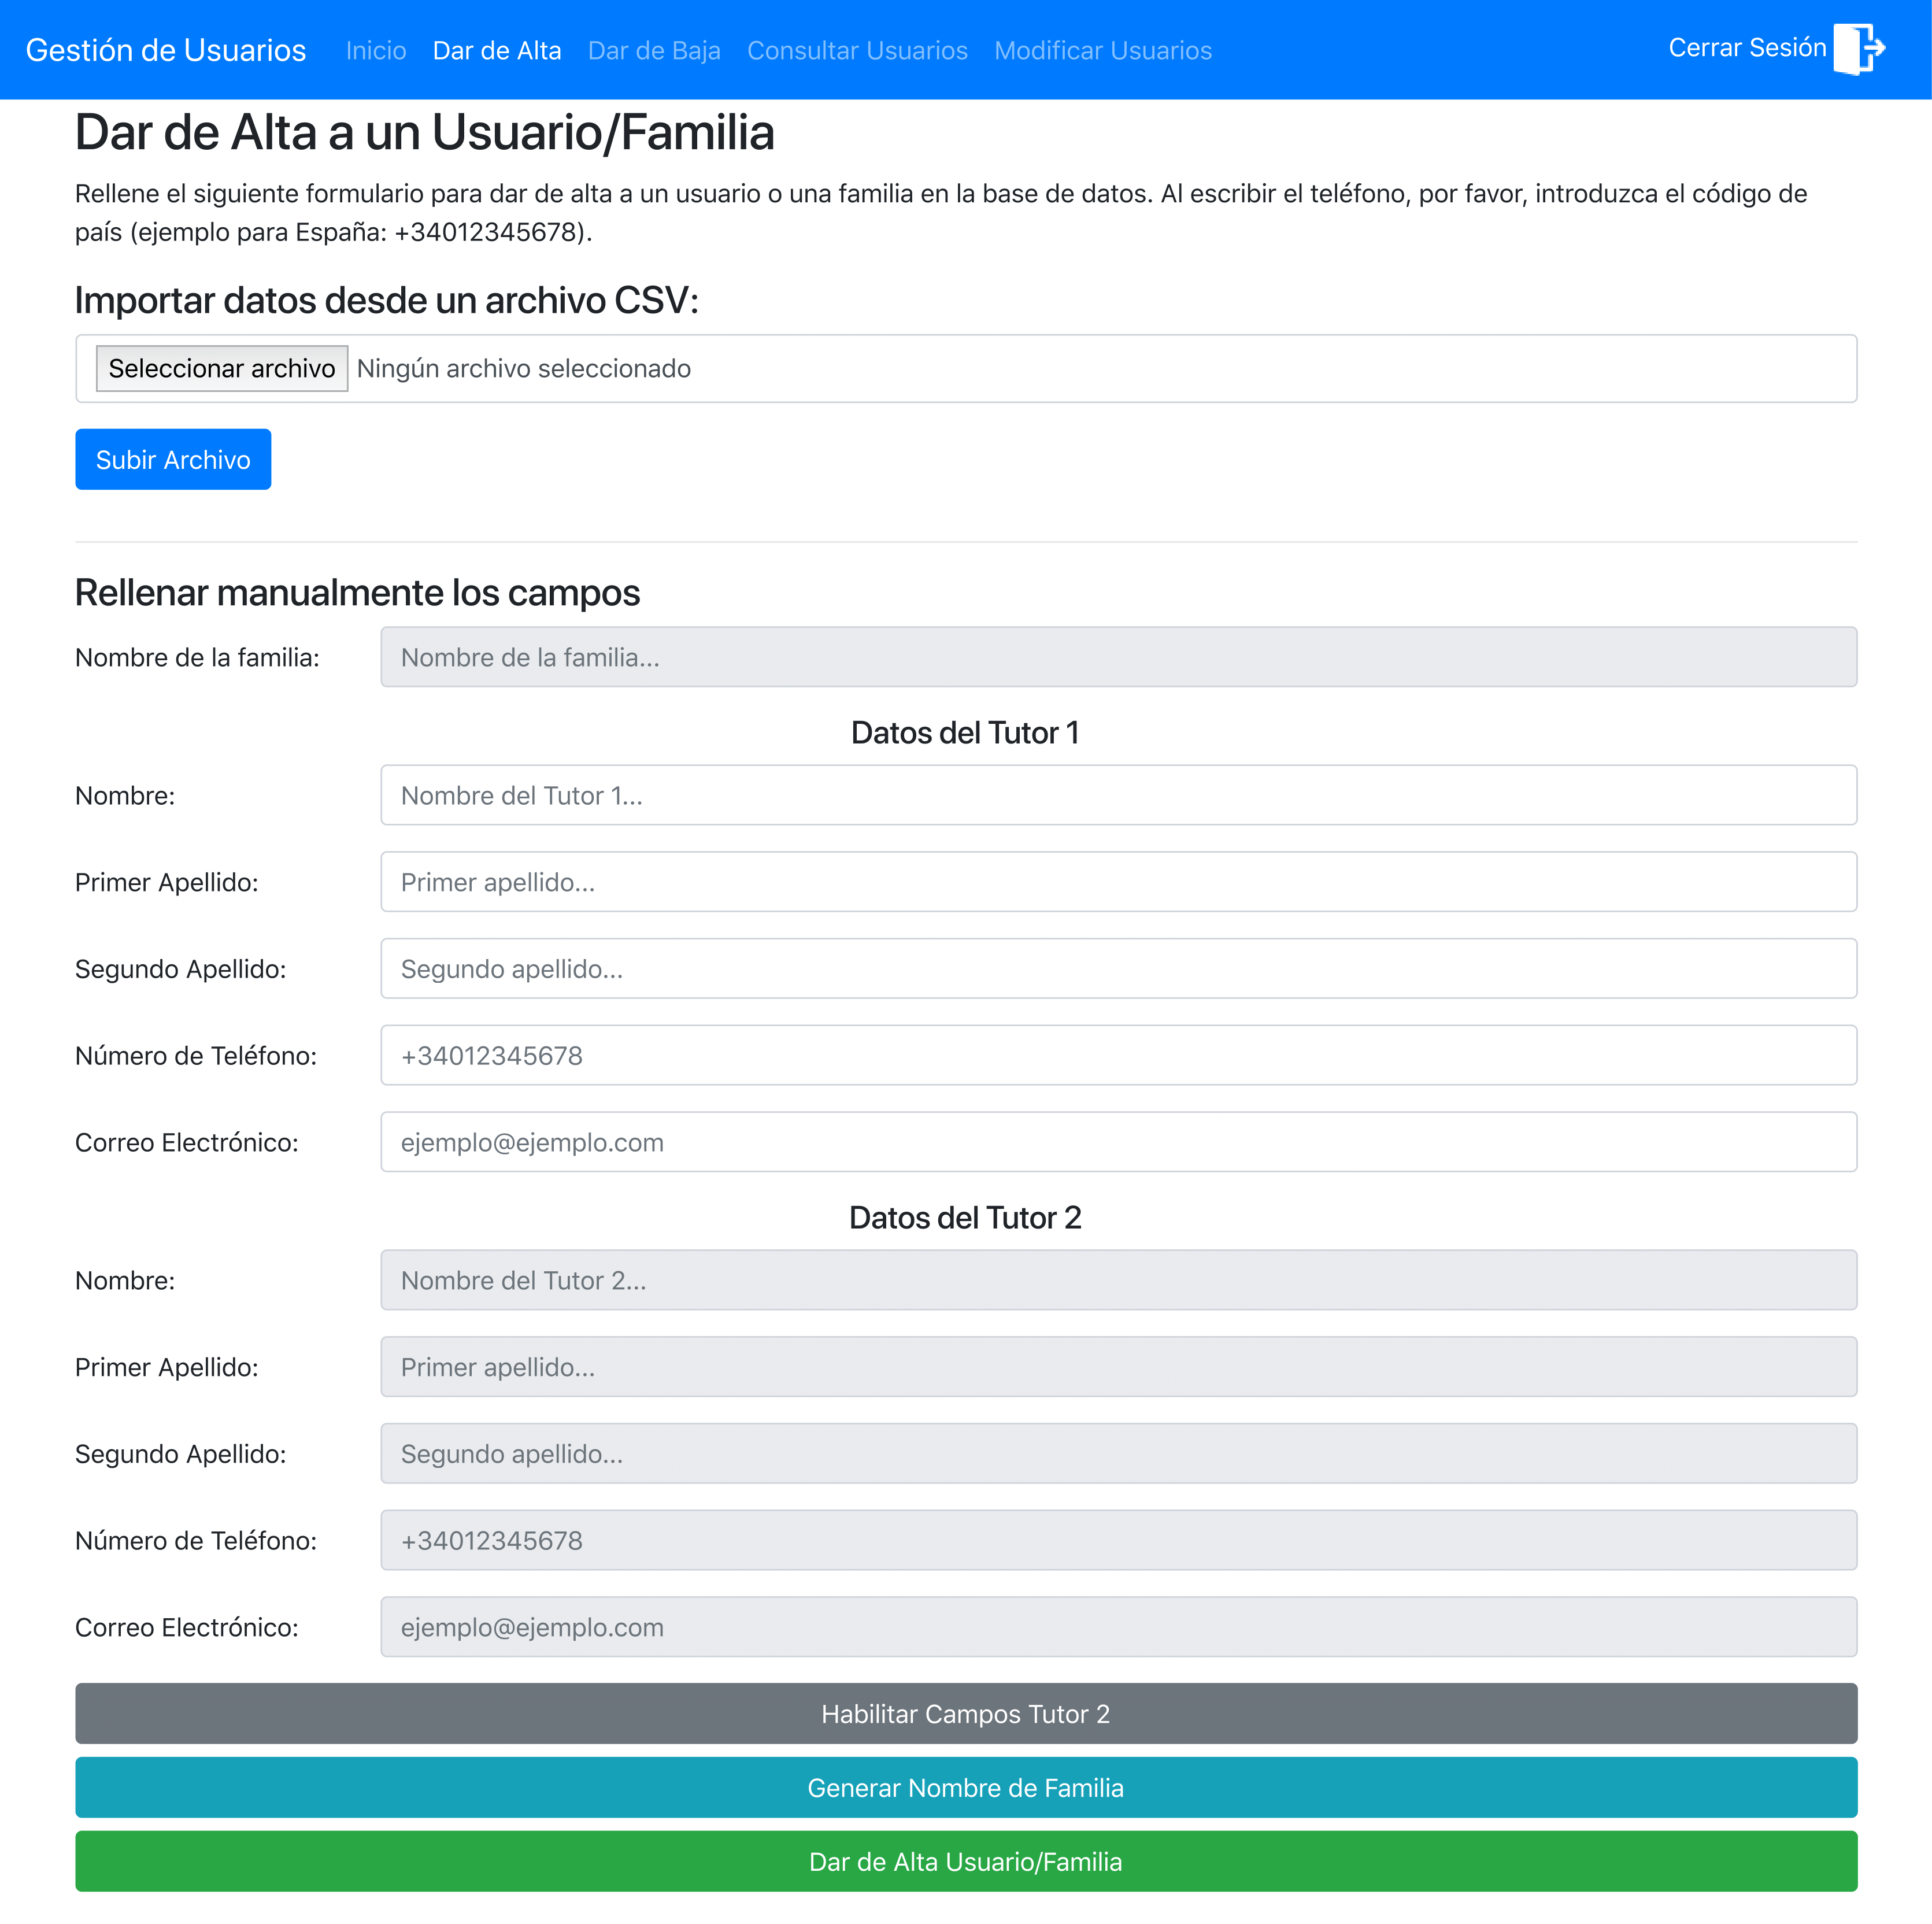
\includegraphics[width=0.75\textwidth]{/manuales/administrador/alta}
		\caption{Página para Dar de Alta a Nuevos Usuarios}
		\label{fig:altaweb}
	\end{center}
\end{figure}

\clearpage

\subsection*{Dar de Baja}
La página para dar de baja a una familia muestra una lista desplegable con una tabla. En dicha lista se encontrarán todos los identificadores de las familias registradas en la base de datos. Al seleccionar uno de ellos, se rellena la tabla con los datos y, al pulsar sobre el botón <<Dar de Baja Usuario/Familia>>, se eliminará la familia seleccionada de la base de datos (Figura \ref{fig:bajaweb}).

\begin{figure}[!h]
	\begin{center}
		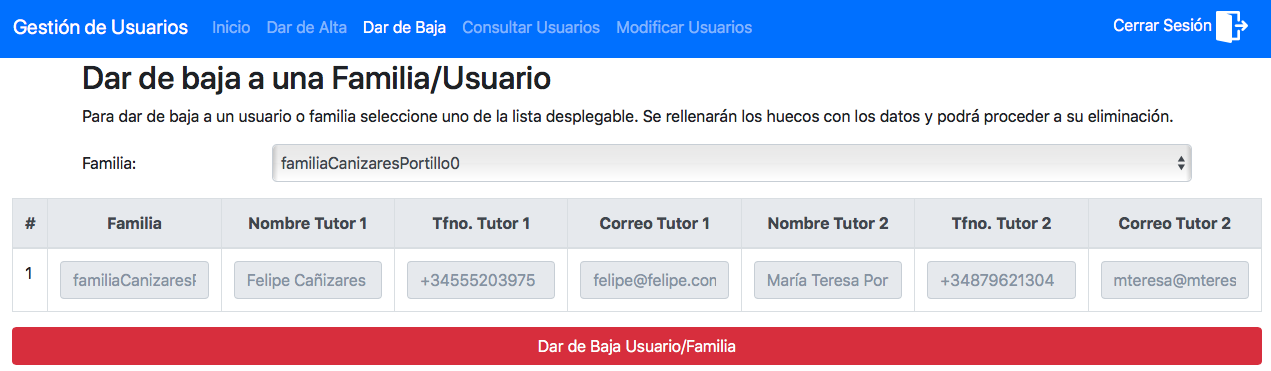
\includegraphics[width=0.8\textwidth]{/manuales/administrador/bajafamilia}
		\caption{Página de Baja de Familias}
		\label{fig:bajaweb}
	\end{center}
\end{figure}

\subsection*{Consultar Usuarios}
La página Web de gestión también permite realizar consultas acerca de las familias que se encuentran registradas. Para ello, en el apartado correspondiente de la misma, se ofrece un filtro para buscar de acuerdo a los diferentes campos. Es decir, se puede introducir un <<texto a buscar>> y seleccionar sobre qué campo se quiere hacer la consulta mediante la lista desplegable. En el caso de que se quiera ver de un vistazo todas las familias registradas en la base de datos, se deberá dejar el campo de <<texto a buscar>> en blanco y pulsar sobre el botón <<Buscar>> (Figura \ref{fig:consultaweb}).

\begin{figure}[!h]
	\begin{center}
		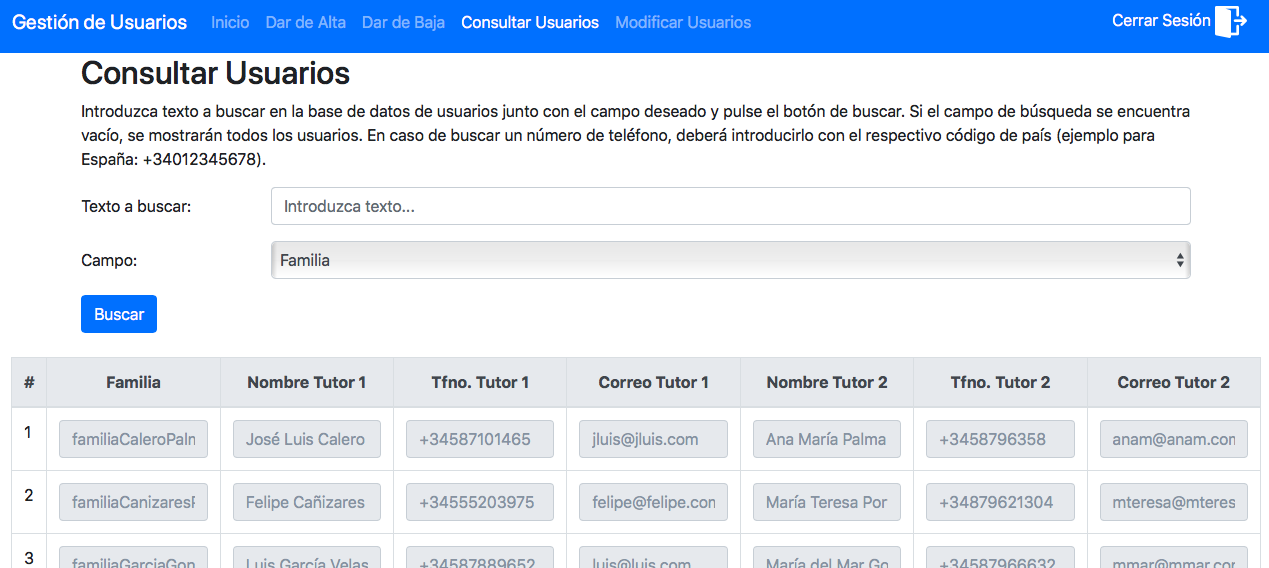
\includegraphics[width=0.85\textwidth]{/manuales/administrador/consulta}
		\caption{Página de Consulta}
		\label{fig:consultaweb}
	\end{center}
\end{figure}

\clearpage

\subsection*{Modificar Usuarios}
Por último, la funcionalidad de modificar usuarios permite cambiar los datos de las familias que están registradas en la base de datos sin la necesidad de eliminar por completo el registro y crearlo de nuevo. Al acceder a la página se muestra una lista desplegable con todos los registros y, seleccionando uno de ellos, se cargan automáticamente todos los datos asociados al mismo en los campos que se encuentran debajo de dicha lista de manera que se pueda visualizar previamente lo que se desea cambiar. Al pulsar el botón <<Modificar Usuario/Familia>> se habilitan todos los campos para su modificación. Una vez que se haya finalizado dicha modificación de datos, se deberá hacer clic sobre el botón anterior, que ahora mostrará <<Confirmar Modificación>> o, si se desea anular el proceso, se hará clic sobre el botón rojo <<Cancelar>>, volviendo a bloquear todos los campos y no afectando ningún cambio en la base de datos (Figura \ref{fig:modificarweb}).

\begin{figure}[!h]
	\begin{center}
		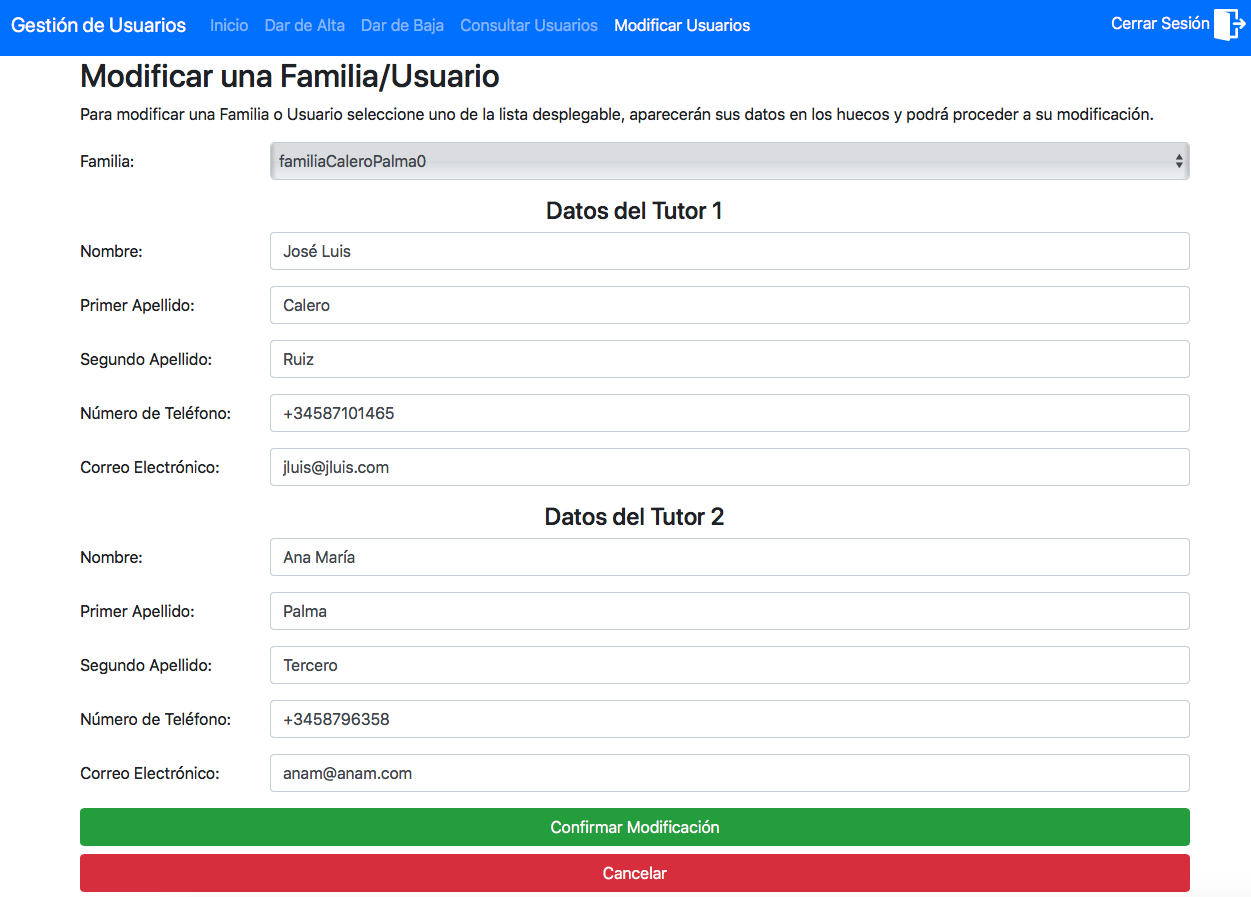
\includegraphics[width=0.85\textwidth]{/manuales/administrador/modificar}
		\caption{Página de Modificación de Usuarios}
		\label{fig:modificarweb}
	\end{center}
\end{figure}